%versi 2 (8-10-2016)
\lstset{
  basicstyle=\ttfamily,
  columns=fullflexible,
  frame=single,
  breaklines=true,
  postbreak=\mbox{\textcolor{red}{$\hookrightarrow$}\space},
}

\chapter{Landasan Teori}
\label{chap:teori}
\setcounter{secnumdepth}{3}


\section{BlueTape}
\paragraph{} Aplikasi \textit{Blue Tape} adalah perangkat lunak \textit{open source} sederhana yang memiliki tujuan utama untuk mengubah berbagai pekerjaan \textit{paper-based} di FTIS UNPAR menjadi \textit{paperless}. Selain itu perangkat lunak ini memiliki beberapa kegunaan lainnya seperti mengautentikasi mahasiswa dan staf UNPAR via OAuth 2.0 ke Google (layanan OAuth ke Google ini juga dapat digunakan untuk menentukan hak akses yang bisa dilihat dari email pengguna) dan \textit{Pilot Project} untuk permohonan transkrip ke Tata Usaha . Aplikasi ini merupakan aplikasi berbasis web dengan memanfaatkan \textit{Codeigniter} dan \textit{Zurb Foundation}. 

Perangkat lunak \textit{Blue Tape} ini didesain sebagai \textit{framework} yang terdiri dari beberapa layanan yang dipisahkan ke dalam modul-modul. Pemisahan layanan ke dalam modul-modul dibuat dengan tujuan agar pemeliharan perangkat lunak lebih mudah dan juga mempermudah cara untuk menambahkan layanan baru ke dalam BlueTape. Sudah ada layanan yang aktif di BlueTape saat ini yaitu \textit{Transcript Request / Manage} yang memiliki fungsi untuk melakukan permohonan serta pencetakan transkrip mahasiswa.



\section{CodeIgniter}
\label{sec:CodeIgniter}  
CodeIgniter adalah \textit{framework} pengembangan aplikasi untuk \textit{developer} yang membangun situs web menggunakan PHP. Tujuannya adalah untuk memungkinkan Anda mengembangkan proyek lebih cepat, daripada bila \textit{developer} menulis kode dari awal, dengan menyediakan banyak kumpulan \textit{library} untuk tugas-tugas yang sering dibutuhkan dan juga menyediakan tampilan sederhana serta struktur logika untuk mengakses \textit{library-library} tersebut. CodeIgniter memungkinkan \textit{developer} untuk fokus secara kretif pada proyek \textit{developer} dengan cara meminimalkan jumlah kode yang dibutuhkan untuk setiap tugas yang diberikan. \cite{CodeIgniter:17}
\\
\\
CodeIgniter dirancang untuk memenuhi kebutuhan :
\begin{itemize}
		\item \textit{Framework} dengan tapak keberadaan yang kecil
		\item performa yang baik
		\item kompabilitas akun \textit{hosting} yang luas yang dapat berjalan di berbagai versi dan konfigurasi PHP
		\item \textit{Framework} yang hampir tidak membutuhkan konfigurasi
		\item \textit{Framework} yang tidak membutuhkan \textit{command line}
		\item \textit{Framework} yang tidak mengikuti aturan pengkodean yang ketat
		\item membutuhkan solusi yang sederhana
		\item dokumentasi yang menyeluruh
	\end{itemize}
	
\subsection{\textit{System Requirements} Server Untuk Menjalankan CodeIgniter}
Server disarankan sudah menggunakan PHP versi 5.6 atau versi-versi setelahnya. CodeIgniter dapat berjalan pada PHP versi lama , namun ada kemungkinan muncul masalah-masalah yang berkaitan dengan performa dan keamanan. \cite{CodeIgniter:17}

\textit{Database} yang didukung oleh CodeIgniter adalah sebagai berikut :
\begin{itemize}
	\item MySQL (5.1+) melalui mysql , mysqli dan pdo drivers
	\item Oracle melalui oci8 dan pdo drivers
	\item PostgreSQL melalui postgre dan pdo drivers
	\item MS SQL melalui mssql, sqlsrv (versi 2005 dan setelahnya) dan pdo drivers
	\item SQLite melalui sqlite (versi 2), sqlite3 (versi 3) dan pdo drivers
	\item CUBRID melalui cubrid dan pdo drivers
	\item Interbase/Firebird melalui ibase dan pdo drivers
	\item ODBC melalui odbc dan pdo drivers
\end{itemize}

\subsection{Cara Instalasi CodeIgniter}
Instalasi CodeIgniter dilakukan dalam 4 langkah :
\begin{itemize}
	\item \textit{Unzip package} CodeIgniter tersebut \cite{CodeIgniter:17}
	\item Unggah folder CodeIgniter dan data-datanya ke dalam server. Pada umumnya \textit{index.php} berada pada \textit{root} server.\cite{CodeIgniter:17}
	\item Buka \textit{application/config/config.php} menggunakan program pengolah teks dan tentukan URL-nya. Jika akan digunakan enkripsi, tentukan kunci enkripsinya.\cite{CodeIgniter:17}
	\item Jika \textit{database} akan digunakan, buka \textit{application/config/database.php} menggunakan program pengolah teks dan atur \textit{database} anda.\cite{CodeIgniter:17}
\end{itemize}

\subsection{Cross-site Request Forgery (CSRF) }
\paragraph{} Perlindungan terhadap CSRF dapat dilakukan dengan cara mengubah nilai variabel berikut menjadi TRUE pada file \textbf{application/config/config.php} \cite{CodeIgniter:17}
\begin{lstlisting}
	$config['csrf_protection'] = TRUE;
\end{lstlisting}
Jika \textit{form helper} digunakan di view aplikasi, maka field csrf akan secara otomatis dimasukan ke dalam form tersebut. Kode dibawah ini akan secara otomatis dimasukan oleh CodeIgniter ketika form\_open() dipanggil.
\begin{lstlisting}
	<input type="hidden" name="<?=$csrf['name'];?>" value="<?=$csrf['hash'];?>" />
\end{lstlisting}
Token dapat diatur agar selalu meregenerasi setiap terjadi \textit{submission} atau juga dapat diatur agar selalu tetap sama sepanjang masa hidup \textit{cookie} CSRF-nya. Regenerasi token akan membuat keamanan sistem lebih kuat, namun dapat menyebabkan masalah navigasi web (seperti navigasi \textit{back/forward} halaman ke halaman, membuka tab baru , dan lain-lain). Regenerasi token dapat diatur dengan mengubah nilai variabel : \cite{CodeIgniter:17}
\begin{lstlisting}
	$config['csrf_regenerate'] = TRUE;
\end{lstlisting}
\subsection{Model-View-Controller}
CodeIgniter didasari pola pengembangan \textit{Model-View-Controller} atau MVC. MVC memisahkan logika aplikasi dengan tampilannya. \cite{CodeIgniter:17}
\begin{itemize}
		\item \textbf{\textit{Model}} merepresentasikan struktur data. Pada umumnya kelas-kelas model menampung fungsi-fungsi untuk mengambil, memperbarui atau memasukan data ke dalam basis data.
		\item \textbf{\textit{View}} menampilkan informasi ke pengguna. 
		\item \textbf{\textit{Controller}} berfungsi sebagai perantara antara model dan view.
\end{itemize}

\subsection{Controller}
Sebuah \textit{controller} adalah kelas yang dinamakan demikian agar dapat diasosiasikan dengan URI.
sebagai contoh URI "example.com/index.php/blog/" , CodeIgniter akan mencari \textit{controller} bernama Blog.php dan menjalankannya. Nama \textit{controller} harus diawali dengan huruf kapital. Selain itu \textit{controller} juga harus  \textit{extend} kelas "CI\_Controller". \cite{CodeIgniter:17} \\ 
Contoh yang benar :
\begin{lstlisting}
	<?php
	class Blog extends CI_Controller {

	}
\end{lstlisting}

Contoh yang salah :
\begin{lstlisting}[language=PHP]
	<?php
	class blog extends CI_Controller {

	}
\end{lstlisting}
	\subsubsection{Method}
	Untuk menjalankan suatu method, maka developer perlu menuliskannya pada segmen kedua URI. Contoh "example.com/index.php/blog/comments" maka akan dijalankan method comments() pada controller blog.php. Method yang akan dijalankan bila bagian kedua URI kosong adalah method index(). Jika URI mengandung lebih dari dua segment, segment-segment tersebut akan dimasukan ke dalam method sebagai parameter. \cite{CodeIgniter:17}
	
	\subsubsection{Default Controller}
	CodeIgniter dapat diperintahkan untuk menjalankan \textit{default controller} jika tidak terdapat URI, pada umumnya terjadi ketika hanya terdapat permintaan menggunakan URL dasar \textit{website}. Penentuan \textit{default controller} terdapat pada \textit{file} "application/config/routes.php" dan set variabel . Nama \textit{controller} tersebut adalah 'blog', maka ketika index.php dijalankan tanpa menspesifikasikan URI akan dijalankan \textit{controller} 'blog'.\cite{CodeIgniter:17}
	
	\subsubsection{Memproses Output}
	CodeIgniter memiliki kelas \textit{output} yang mengurus pengiriman data ke \textit{web browser} secara otomatis. Untuk kasus-kasus saat pengguna ingin mengubah cara pengiriman data tersebut, CodeIgniter menyediakan caranya dengan menambahkan method bernama "\_output()" ke \textit{controller} terkait. Jika controler memiliki method bernama "\_output()" maka controller tersebut akan  selalu dipanggil oleh kelas "output".\cite{CodeIgniter:17} \\
Contoh penggunaan method "\_output()" : 
\begin{lstlisting}
	public function _output(\$output)
	{
        echo $output;
	}
\end{lstlisting}

	\subsubsection{Private Method}
	Method-method dengan tipe \textit{private} tidak dapat diakses oleh publik. Method ini hanya dapat diakses oleh method lain dalam \textit{controller} yang sama. Selain it           u method ini juga tidak akan dapat diakses melalui URL.\cite{CodeIgniter:17}\\
Contoh penulisan \textit{private method}:
\begin{lstlisting}
	private function _utility()
	{
        // kode program
	}
\end{lstlisting}
Method di atas tidak dapat diakses dengan cara pemanggilan method pada umumnya seperti :
\begin{lstlisting}
	example.com/index.php/blog/_utility/
\end{lstlisting}

	\subsubsection{Mengorganisir Controller-controller ke Dalam Sub Direktori}
\paragraph{} Di CodeIgniter pengguna dapat mengorganisir \textit{controller-controller} ke dalam sub direktori. Untuk melakukannya cukup dengan membuat sub direktori di dalam direktori \textit{application/controllers/} dan simpan kelas-kelas \textit{controller} ke dalamnya. Ketika menggunakan fitur ini, pengguna harus menspesifikasikan foldernya ke dalam URI.\cite{CodeIgniter:17} \\
Contoh ada controller yang berlokasi di:
\begin{lstlisting}
	application/controllers/products/Shoes.php
 \end{lstlisting}
Untuk memanggil controller tersebut URI harus menuliskan nama sub direktorinya :
\begin{lstlisting}
	example.com/index.php/products/shoes/show/123
\end{lstlisting}

\subsection{View}
\textit{View} adalah sebuah halaman web, bagian-bagian halaman ( seperti \textit{header, footer, sidebar}, dan-lain-lain) atau bagian dari \textit{view} lainnya. \textit{View} tidak pernah dipanggil secara langsung, melainkan harus melalui controller karena dalam framework MVC controller berfungsi sebagai pengatur.\cite{CodeIgniter:17} \\
Controller dapat memanggil view menggunakan potongan kode seperti di bawah ini :
\begin{lstlisting}
	$this->load->view('name');
\end{lstlisting}
Jika 1 halaman terdiri dari beberapa view, CodeIgniter juga menyediakan cara untuk memanggil banyak view sekaligus:
\begin{lstlisting}
	<?php

	class Page extends CI_Controller {

       	 public function index()
       	 {
        	     $data['page_title'] = 'Your title';
        	     $this->load->view('header');
        	     $this->load->view('menu');
       	         $this->load->view('content', $data);
       	         $this->load->view('footer');
       	 }

	}
\end{lstlisting}
BIla ada data lain yang akan dikirimkan ke view dari controller, gunakan potongan kode seperti di bawah ini :
\begin{lstlisting}
	$this->load->view('name', $data);
\end{lstlisting}

\subsection{Model}
Model adalah kelas PHP yang dirancang untuk bekerja dengan informasi-informasi di \textit{database}. Sebagai contoh, misalkan CodeIgniter digunakan untuk mengatur sebuah blog maka model mengandung fungsi-fungsi seperti \textit{select, insert, update }data-data blog. \cite{CodeIgniter:17}

\subsubsection{Anatomi dari Model}
Model disimpan di direktori \textbf{application/models}. Model dapat disimpan dalam sub-direktori jika dibutuhkan. Bentuk dasar kode pada kelas model adalah seperti di bawah ini: \cite{CodeIgniter:17}
\begin{lstlisting}
	class Model_name extends CI_Model {
	
		public function_construct()
		{
			parent::_construct();
			//constructor code
		}
	}
\end{lstlisting}
\textbf{Model\_name} adalah nama dari kelasnya. Huruf pertama dari nama kelas harus huruf kapital dengan huruf-huruf setelahnya ditulis menggunakan huruf kecil. Kelas model harus dipastikan meng-\textit{extend} kelas Model dasar. Nama file harus sama dengan nama kelasnya. \cite{CodeIgniter:17}

\subsubsection{\textit{Load} Model}
Pada umumnya model akan di-\textit{load} di dalam method-method \textit{controller}. Untuk \textit{load} model diperlukan method berikut:
\begin{lstlisting}
	$this->model->model('model_name');
\end{lstlisting}
Jika model terdapat pada sub-direktori, perlu dimasukan \textit{path}-nya ke dalam direktori 'models'. Misalnya model terdapat di \textit{application/models/blog/Queries.php} maka untuk \textit{load} model gunakan :
\begin{lstlisting}
	$this->load->model('blog/queries');
\end{lstlisting}
Bila ada sebuah model yang akan digunakan secara global pada aplikasi pengguna, CodeIgniter bisa diperintahkan untuk \textit{auto-load} model tersebut ketika instalasi sistem. Untuk melakukan hal ini, tambahkan model ke dalam \textit{autload array} yang berlokasi di "\textit{application/config/autoload.php}". \cite{CodeIgniter:17}

\subsubsection{Menghubungkan Model Dengan \textit{Database}}
\paragraph{}Ketika Model dipanggil, model tidak akan terhubung ke database secara otomatis. Ada dua cara untuk menghubungkan model dengan \textit{database} : \cite{CodeIgniter:17}
\begin{enumerate}
	\item Menghubungkan secara otomatis ketika instalasi sistem dilakukan menggunakan fitur auto-load seperti disebutkan di bagian \textit{Load} Model di atas.
	\item Menghubungkan \textit{database} secara manual. Untuk menghubungkan \textit{database} dengan model, pengguna perlu untuk memanggil \textit{database}-nya di \textit{controller} atau di \textit{model} itu sendiri dengan menuliskan potongan kode: \cite{CodeIgniter:17}
	\begin{lstlisting}
	$this->load->database();	
	\end{lstlisting}
Parameter-parameter yang tersedia untuk potongan kode di atas adalah:
	\begin{itemize}
	\item Nama dari database yang dituju berupa array atau \textit{Data Source Name}(DSN) string.
	\item \textit{Boolean} untuk menentukan id koneksi perlu dikembalikan ke model atau tidak.
	\item \textit{Boolean} untuk menentukan perlunya dibuat \textit{Query Builder} atau tidak. Jika tidak ditentukan, nilai dari parameter ini adalah TRUE.
	\end{itemize}
\end{enumerate}

\subsection{Kelas Migrasi}
\paragraph{}Kelas ini digunakan untuk memudahkan pengubahan \textit{database} secara terstruktur dan terorganisir dengan baik. Dengan cara ini maka penguna tidak perlu memberi tahu penguna lainnya yang sedang mengembangkan aplikasi yang sama untuk melakukan perubahan \textit{database} secara manual, penguna lain cukup menjalankan kelas migrasi ini. Kelas ini akan secara otomatis membuat tabel bernama "\textit{migration}" di \textit{database} yang mencatat migrasi-migrasi mana saja yang sudah dijalankan, yang perlu dilakukan secara manual oleh pengguna adalah untuk memperbarui \textit{file} aplikasinya dan memanggil \textit{\$this->migration->current()} untuk menentukan migrasi mana yang perlu dijalankan. Untuk mengatur preferensi dari kelas migrasi terdapat di \textbf{aplication/config/migration.php}. \cite{CodeIgniter:17} 
\begin{center}
	\begin{table}[H]
	\begin{tabular}{|c|c|c|p{3cm}|}
 			\hline
		Preferensi & \textit{Default} & Opsi & Deskripsi  \\
			\hline
		 migration\_enabled & FALSE & TRUE / FALSE & Menentukan migrasi dijalankan atau tidak. \\
			 \hline
			 migration\_path & APPPATH.\'migrations/\' & None &	Alamat ke folder migrasi. \\
			 \hline
			 migration\_version & 0 & None & Versi migrasi yang digunakan.\\
			 \hline
			 migration\_table & migrations & None & 	Nama tabel migrasi di \textit{database}. \\
			 \hline
			 migration\_auto\_latest & FALSE & TRUE / FALSE & 	Menentukan dijalankannya migrasi otomatis atau tidak. \\
			 \hline
			  migration\_type & \'timestamp\' & 	\'timestamp\' / \'sequential\' & 	Tipe penomoran kelas migrasi yang digunakan. \\
			 \hline
	\end{tabular}
	\caption{Daftar Preferensi di Kelas Migrasi}
	\end{table}
\end{center}
\subsubsection{Nama Kelas Migrasi}
Setiap migrasi dijalankan sesuai urutan numerik baik dengan urutan menaik atau menurun tergantung dari metode yang digunakan. Ada dua cara penomoran yang bisa dilakukan yaitu :
\begin{itemize}
	\item \textbf{Sekuensial}: setiap migrasi dinomori secara sekuensial, dimulai dengan angka \textbf{001}. Setiap nomor harus terdiri dari 3 digit dan tidak ada jeda di angka tersebut. Cara penomoran ini adalah satu-satunya cara yang digunakan sebelum versi CodeIgniter 3.0 . \cite{CodeIgniter:17}
	\item \textbf{\textit{Timestamp}}: setiap migrasi menggunakan \textit{timestamp} ketika kelas migrasinya dibuat. Format penomrannya adalah YYYYMMDDHHIISS.
		\begin{itemize}
		\item YYYY	: tahun terdiri dari 4 digit
		\item MM	: bulan terdiri dari 2 digit
		\item DD	: hari terdiri dari 2 digit
		\item HH	: jam terdiri dari 2 digit
		\item II	: menit terdiri dari 2 digit
		\item SS	: detik terdiri dari 2 digit
		\end{itemize}
Cara ini digunakan untuk menghindari konflik penomoran ketika bekerja dalam tim. Cara penomoran ini merupakan cara yang lebih banyak digunakan sejak versi CodeIgniter 3.0 dan setelahnya. \cite{CodeIgniter:17}
\end{itemize}
Urutan penomran dapat diatur menggunakan \textit{\$config['migration\_type']} di \textit{file} \textit{application/config/migration.php} . Apapun cara yang dipilih, pisahkan nama file dan penomoran kelasnya menggunakan tanda garis bawah. Sebagai contoh: \cite{CodeIgniter:17}
\begin{itemize}
	\item 001\_add\_blog.php (penomoran sekuensial)
	\item 20121031100537\_add\_blog.php (penomoran dengan \textit{timestamp})
\end{itemize}

\subsection{Flow Chart Codeignter}
Gambar dibawah mengilustrasikan aliran data dalam sistem : \footnote{https://www.codeigniter.com/userguide3/overview/appflow.html} 
\begin{figure} [H]
	\centering  
	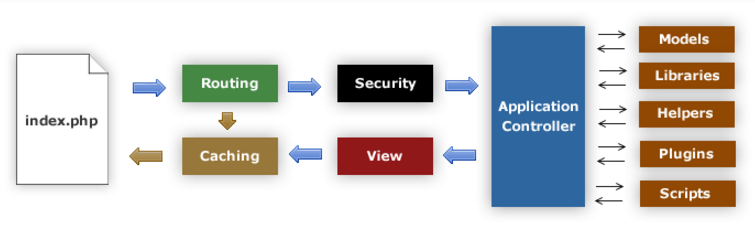
\includegraphics[scale=0.7]{appflowchart.png}  
	\caption[Flow Chart Codeignter]{Flow Chart Codeignter} 
	\label{fig:flow-chart-CodeIgniter} 
\end{figure}

\begin{enumerate}
		\item index.php berfungsi sebagai controller depan. Menginisialisasi sumber daya yang dibutuhkan untuk menjalankan CodeIgniter
		\item Router memeriksa permintaan HTTP untuk menentukan apa yang akan dilakukan pada permintaan tersebut.
		\item Jika ada cache file, maka akan dikirim langsung ke browser. Melewati cara eksekusi sistem yang normal.
		\item Security. Sebelum controller aplikasi dimuat, permintaan HTTP dan data-data pengguna yang telah diserahkan disaring untuk kemanan.
		\item Controller memuat model, pustaka inti (\textit{core libraries}), pembantu dan sumber daya lain yang dibutuhkan untuk memproses permintaan khusus.
		\item Kemudian tampilan akhir dibuat dan dikirim ke web browser untuk dilihat. Jika caching diaktifkan, maka tampilan dimasukan ke dalam cache terlebih dahulu sehingga pada permintaan selanjutnya tampilan tersebut dapat diakses lebih cepat.
	\end{enumerate}

\section{phpMyAdmin}
\paragraph{} phpMyAdmin dapat mengatur keseluruhan server MySQL (membutuhkan \textit{super-user}) dan juga satu basis data. Untuk mengatur satu basis data, dibutuhkan pengaturan \textit{user} MySQL yang hanya dapat membaca/menulis database yang ditentukan.\cite{phpmyadmin:17} \\ 
Fitur yang didukung :
\begin{itemize}
	\item \textit{browse} dan \textit{drop} basis data.
	\item menampilkan hasil pencarian \textit{query}.
	\item membuat, menduplikasi, menghapus, mengubah nama basis data, tabel, kolom dan indeks.
	\item memelihara server, basis data dan tabel.
	\item mengeksekusi, mengubah, dan \textit{bookmark} laporan SQL.
	\item memuat file teks ke dalam tabel. \cite{phpmyadmin:17}
	\item membuat dan membaca \textit{dump} dari tabel.
	\item mengeskpor data ke berbagai format: CSV, XML, PDF, ISO/IEC 26300 - OpenDocument Text and Spreadsheet, Microsoft Word 2000 dan format LATEX.
	\item mengimpor data dan struktur MySQL dari CSV, XML, PDF dan ISO/IEC 26300 - OpenDocument Text and Spreadsheet.
	\item mengatur banyak server.
	\item mengatur pengguna MySQL dan hak aksesnya.
	\item memeriksa integritas tabel MyISAM.
	\item memakai \textit{Query-by-example }(QBE) untuk membuat \textit{query} kompleks yang menghubungkan tabel-tabel.
	\item membuat grafik PDF dari basis data.
	\item Mencari secara global di dalam basis data.
	\item mengubah data yang disimpan di basis data ke dalam format apapun berdasarkan fungsi yang sudah ditentukan pengguna. Misalnya menampilkan data BLOB sebagai gambar atau \textit{link} pengunduhan.
	\item mencatat perubahan-perubahan basis data, tabel dan \textit{view}.
	\item mendukung tabel InnoDB dan \textit{foreign key}. \cite{phpmyadmin:17}
	\item mendukung mysqli dan ekstensi MySQL.
	\item menambah, mengubah, memanggil, mengekspor dan menghapus prosedur dan fungsi yang disimpan.
	\item menambah, mengubah, mengekspor dan menghapus \textit{events} dan \textit{triggers}.
	\item tersedia dalam 80 bahasa berbeda.
\end{itemize}

\section{Cross Site Request Forgery}
\paragraph{}"Cross Site Request Forgery" atau "Session Riding" adalah teknik penyerangan yang mengeksploitasi otentikasi implisit. Penyerangan ini dilakukan dengan cara menyebabkan browser korban membuat \textit{http requests} tersembunyi ke sumber daya - sumber daya terlarang. Pada kasus ketika \textit{request} untuk sumber daya tersebut berhasil, akan menyebabkan browser atau aplikasi web terkait untuk melakukan tindakan-tindakan penyerangan tersebut secara terus menerus. Penyerangan ini bertujuan untuk berbagai hal seperti mengubah \textit{field-field} di dalam \textit{database}, mengirim email atau mengubah bagian-bagian aplikasi. Semua aksi tersebut dilakukan menggunakan token otentikasi milik korban. \cite{barth08csrf}

\paragraph{}Pada umumnya \textit{web browser} memiliki kebijakan untuk memperbolehkan \textit{website-website} untuk mengirim \textit{HTTP request} ke alamat jaringan manapun. Akibat dari kebijakan ini, maka penyerang dapat mengendalikan konten-konten yang dianggap oleh \textit{browser} bukan di bawah kendali pengguna. Konten yang dapat dikendalikan oleh penyerang diantaranya : \cite{barth08csrf}
\begin{itemize}
	\item \textbf{Konektivitas Jaringan}. Misalnya bila korban menggunakan \textit{firewall}, maka penyerang dapat mempengaruhi browser pada mesin korban untuk mengirim \textit{network request} ke mesin-mesin lain yang menggunakan firewall juga yang tidak dapat diakses secara langsung melalui mesin milik penyerang.
	\item \textbf{Membaca Status Browser}. \textit{Request-request} yang dikirimkan ke jaringan melalui \textit{browser} pada umumnya berisi status browser seperti cookies, sertifikat klien atau data otentikasi sederhana.
	\item\textbf{ Menulis Status Browser}. Penyerang membuat \textit{browser} untuk menulis \textit{network request}. \textit{Browser} juga akan bereaksi pada respon dari website yang dituju. Hal ini mengakibatkan \textit{browser} memodifikasi beberapa bagian status browser.
\end{itemize}

\paragraph{}Serangan CSRF tidak terbatas pada satu \textit{request} palsu saja. Alur kerja yang membutuhkan serangkaian \textit{request} http juga rentan terhadap serangan ini selama kondisi-kondisi yang diperlukan terpenuhi. Misalnya bila setiap konten dan \textit{identifier} dalam setiap langkah pada alur kerja \textit{web form} diketahui dan alur kerja dari \textit{website} tersebut tidak memiliki mekanisme lain untuk melacak cara kerja langkah per-langkah \textit{web form}-nya, melainkan hanya menggunakan \textit{identifier} dari \textit{session} saja. Jika kondisi tersebut dipenuhi, maka penyerang dapat membuat serangkaian \textit{iframe-iframe} tersembunyi yang mengandung \textit{web form} berbahaya. \textit{Form-form} tersebut lalu dikirimkan secara sekuensial melalui JavaScript menggunakan \textit{event} \textit{onload} dari \textit{iframe} untuk membuat server yang menerimanya mengira bahwa \textit{form-form} tersebut diisi oleh user dengan benar. \cite{JohnsWinter2006}

\section{Zurb Foundation}
\label{zurbfoundation}

\paragraph{}  Foundation adalah kumpulan pola desain HTML, CSS dan Javascript yang dapat digunakan untuk membuat website. Hal tersebut untuk membantu \textit{developer} agar tidak perlu menulis kode yang sama berulang kali. Selain membantu mengehemat waktu, Foundation juga membantu \textit{developer} untuk menulis kode dengan lebih baik. Foundation dapat bekerja pada berbagai media seperi komputer desktop, laptop, tablet, dan telepon genggam.\cite{zurbfoundation:17} \\
Komponen-komponen dalam Foundation sendiri ada beberapa macam diantarnya sebagai berikut:

\begin{itemize}
	\item  Grid untuk mempermudah pembagian halaman.\footnote{\label{note2}http://foundation.zurb.com/sites/docs/v/5.5.3/}
	\item  Desain tombol yang bermacam-macam. Desain tombol ini dapat diubah-ubah dengan cara menambahkan kelas.\textsuperscript{\ref{note2}}
	\item  Navigasi untuk mempermudah pengunjung aplikasi dalam menggunakan aplikasinya.\textsuperscript{\ref{note2}}
	\item  Plugins JavaScript untuk mempermudah \textit{developer} dalam membuat tampilan aplikasinya.\textsuperscript{\ref{note2}}
\end{itemize}

\subsection{Top Bar}
\paragraph{} Top bar adalah \textit{wrapper} sederhana untuk komponen-komponen menu website. Top bar dapat memiliki 2 bagian yaitu bagian kiri \textbf{(.top-bar-left)} dan bagian kanan \textbf{(.top-bar-right)}. Pada layar yang kecil bagian top bar ini bisa menjadi di atas atau di bawah sisi lainnya. .\cite{zurbfoundation:17} 

\subsection{Reveal Modal}
\paragraph{} Pada dasarnya modal hanyalah sebuah kontainer kosong, jadi pengguna dapat memasukan konten apapun ke dalamnya. Untuk membuat modal, buat kelas \textbf{.reveal} dan atribut \textbf{data-reveal} lalu beri id unik ke kontainernya tersebut seperti contoh di bawah ini : .\cite{zurbfoundation:17} 
\begin{lstlisting}
<div class="reveal" id="exampleModal1" data-reveal>
  		...
</div>	
\end{lstlisting}
Untuk membuka modal, tambahkan atribut \textbf{data-open} ke elemen apapun. Nilai dari \textbf{data-open} adalah id dari modalnya.
\begin{lstlisting}
<p><button class="button" data-open="exampleModal1">Click me for a modal</button></p>
\end{lstlisting}
Jika tidak diberi aturan tambahan, pada dasarnya modal akan ditutup jika pengguna menekan area di luar dari modal atau ketika tombol ESC ditekan. Untuk memberi tombol "\textit{close}" di menu modal tambahkan atribut \textbf{data-close} ke elemen yang berisi pemicu modal. Contoh dapat dilihat pada potongan kode di bawah. .\cite{zurbfoundation:17} 
\begin{lstlisting}
<button class="close-button" data-close aria-label="Close modal" type="button">
  <span aria-hidden="true">&times;</span>
</button>
\end{lstlisting}

\subsection{Variabel Sass \textit{Reveal Modal}}
Berikut adalah variabel-variabel yang dapat digunakan untuk mengkostumisasi modal :
\begin{center}
	\begin{table}[H]
	\begin{tabular}{|c|c|c|p{3cm}|}
 				\hline
			Nama & Tipe & Nilai \textit{Default} & Deskripsi  \\
				\hline
			 \$reveal-background & Color & \$white & Warna \textit{default} latar belakang modal \\
			 	\hline
			  \$reveal-width & Number & 600px & Lebar \textit{default} modal, tanpa memakai kelas apapun \\
				 \hline
			  \$reveal-max-width & Number & \$global-width & Lebar maximum modal \\
				 \hline
			 \$reveal-padding & Number & \$global-padding & \textit{Default} padding di dalam modal \\
			 	\hline
			  \$reveal-border & Number & \$global-radius & Nilai \textit{default} radius untuk sebuah modal \\
			 	\hline
			  \$reveal-zindex & Number & 1005 & nilai z-index untuk modal. \\
			 	\hline
			 	\$reveal-overlay-background & Color & rgba(\$black,0,45) & Warna latar belakang penutup modal \\
			 	\hline
	\end{tabular}
	\caption{Daftar Variabel Sass Untuk \textit{Reveal Modal}}
	\end{table}
\end{center}

\subsection{Scrolling Table}
Scrolling table diguanakan bila banyak data yang ada pada tabel. Dengan menggunakan ini maka isi tabel dapat digeser secara horizontal. Untuk menggunakan tabel jenis ini, deklarasikan kelas \textbf{table-scroll} seperti contoh di bawah:
\begin{lstlisting}
<div class="table-scroll">
  <table></table>
</div>
\end{lstlisting}

\subsubsection{Variabel Sass Untuk Tabel}
Berikut adalah daftar variabel Sass yang dapat dikustomisasi untuk mengubah tampilan komponen-komponen dari tabel 
\begin{center}
	\begin{table}[H]
	\begin{tabular}{|c|c|p{4cm}|p{5cm}|}
 				\hline
			Nama & Tipe & Nilai \textit{Default} & Deskripsi  \\
				\hline
			 \$table-background & Color & \$white & Warna \textit{default} tabel \\
			 	\hline
			  \$table-color-scale & Number & 5\% & Skala warna gelap pada tabel bergaris\\
				 \hline
			  \$table-border & List & 	1px solid smart-scale(\$table-background, \$table-color-scale) & Tipe batas tabel yang digunakan \\
				 \hline
			 \$table-padding & Number & rem-calc(8 10 10) & \textit{Default} padding di tabel \\
			 	\hline
			  \$table-hover-scale & Number & 2\% & Skala warna gelap baris tabel ketika ditunjuk kursor \\
			 	\hline
			  \$table-row-hover & List & darken(\$table-background, \$table-hover-scale) & Warna baris pada tabel ketika ditunjuk oleh kursor. \\
			 	\hline
			 	\$table-row-stripe-hover & List & darken(\$table-background, \$table-color-scale + \$table-hover-scale) & Warna  baris gelap pada tabel bergaris ketika ditunjuk kursor \\
			 		\hline
			 	\$table-is-striped & Boolean & TRUE & Jika bernilai TRUE maka tabel menggunakan tipe tabel bergaris \\
			 		\hline
			 	\$table-striped-background & Color & smart-scale(\$table-background, \$table-color-scale) & Warna baris gelap pada tabel bergaris \\
			 		\hline
			 	\$table-stripe & Keyword & even & Nilai untuk memunculkan baris gelap pada tabel, kecuali pada bagian \textit{header}. Jika bernilai \textit{even}, maka baris genap akan memiliki warna latar. Jika bernilai \textit{odd} maka baris ganjil yang akan memiliki warna latar \\
			 	\hline
			 	\$table-head-background & Color & smart-scale(\$table-background, \$table-color-scale / 2) & Warna latar belakang \textit{header} tabel \\
			 	\hline
			 	\$table-head-row-hover & List & darken(\$table-head-background, \$table-hover-scale) & Warna \textit{header} ketika ditunjuk kursor\\
			 	\hline
			 	\$table-foot-background & Color & smart-scale(\$table-background, \$table-color-scale) & Warna latar belakang \textit{footer} \\
			 	\hline
			 	\$table-foot-row-hover & List & darken(\$table-foot-background, \$table-hover-scale) & Warna latar belakang \textit{footer} ketika ditunjuk kursor \\
			 	\hline
			 	\$table-head-font-color & Color & \$body-font-color & Warna teks yang berada di \textit{header} \\
			 	\hline
			 	\$table-foot-font-color & Color & \$body-font-color & Warna teks yang berada di \textit{footer} \\
			 	\hline
			 	\$show-header-for-stacked & Boolean & false & Nilai untuk menentukan penggunaan header ketika menggunakan \textit{stacked table} \\
			 	\hline
			 	\$table-stack-breakpoint & Breakpoint & medium & Batas pemicu perubahan jenis tabel dari tipe \textit{mobile} menjadi \textit{desktop} atau sebaliknya \\
			 	\hline
	\end{tabular}
	\caption{Daftar Variabel Sass Untuk Kelas Tabel}
	\end{table}
\end{center}

\section{Google OAuth 2.0} %https://developers.google.com/identity/protocols/OAuth2
\label{googleoauth}

\paragraph{} Google OAuth 2.0 merupakan salah satu protokol dari Google Sign-in. Google OAuth 2.0 digunakan oleh Google API untuk otorisasi dan autentikasi. Secara garis besar, cara pemakaian Google OAuth 2.0 adalah sebagai berikut : \footnote{\label{noteOauth}https://developers.google.com/identity/protocols/OAuth2}

	\begin{enumerate}
  	\item Dapatkan OAuth 2.0 credential dari konsol Google API. OAuth 2.0 credential seperti client ID dan client secret yang diketahui oleh Google dan aplikasi pengguna, dapat didapatkan di halaman https://console.developers.google.com/ .  \textsuperscript{\ref{noteOauth}}
  	\item Dapatkan token akses dari Google Authorization Server. Sebelum aplikasi dapat mengakses data pribadi menggunakan Google API, aplikasi tersebut harus mendapat token akses yang memberikan akses ke API. Satu token akses dapat memberikan berbagai macam akses ke banyak API. Variable parameter "\textit{scope}" mengendalikan kumpulan-kumpulan sumber daya dan operasi yang telah diperbolehkan untuk diakses oleh token akses. Selama masa permintaan token akses, aplikasi mengirimkan satu atau lebih nilai ke dalam parameter "\textit{scope}". Ada beberapa cara untuk melakukan permintaan, tergantung dari tipe aplikasi yang sedang dibuat. Sebagai contoh aplikasi JavaScript dapat meminta token akses menggunakan \textit{redirect} dari \textit{browser} yang mengarah ke Google, sementara aplikasi lain yang terinstall di dalam perangkat yang tidak memiliki browser menggunakan \textit{web service} untuk melakukan permintaan. Beberapa permintaan membutuhkan tahap autentikasi yang meminta pengguna untuk masuk ke akun Google mereka. Setelah masuk ke dalam akun, pengguna akan diminta jika mereka bersedia untuk memberikan izin ke aplikasi yang sedang melakukan permintaan tersebut.\textsuperscript{\ref{noteOauth}}
  	\begin{figure} [H]
	\centering  
	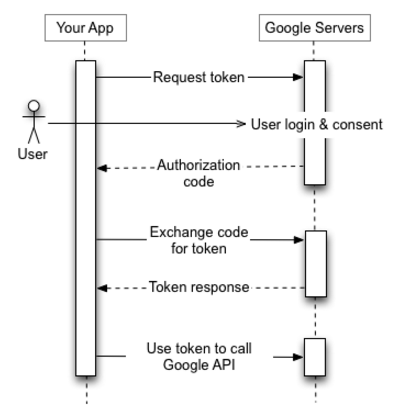
\includegraphics[scale=0.7]{skenario_token.png}  
	\caption[Skenario OAuth menggunakan token akses]{Skenario OAuth menggunakan token akses} 
	\label{fig:skenario-token} 
\end{figure}
  	\item Mengirim akses token ke API. Setelah aplikasi mendapatkan akses token, aplikasi tersebut akan mengirim token ke Google API dalam bentuk HTTP \textit{authorization header}. Jika memungkinkan, aplikasi dapat mengirim token-token sebagai parameter \textit{URI query-string}. Pengiriman dalam bentuk parameter URI tidak disarankan karena parameter URI dapat tersimpan dalam \textit{log} yang tidak aman. Token akses hanya berlaku untuk kumpulan operasi dan sumber daya yang dideskripsikan dalam parameter \textit{scope} di permintaan token. \textsuperscript{\ref{noteOauth}}
	\item Jika dibutuhkan, token akses dapat di-\textit{refresh} karena token akses memiliki masa berlaku terbatas. Jika aplikasi membutuhkan akses ke Google API lebih dari masa berlaku satu buah token, aplikasi dapat mendapatkan token \textit{refresh}. Token \textit{refresh} memungkinkan aplikasi untuk mendapatkan token akses baru.\textsuperscript{\ref{noteOauth}}
  
\end{enumerate}

\section{PHPExcel} 
\label{phpexcel}

\paragraph{} PHPExcel adalah suatu proyek yang menyediakan berbagai kelas-kelas untuk pemrograman bahasa PHP yang memungkinkan \textit{developer} untuk menulis dan membaca dari berbagai macam bentuk \textit{spreadsheet} seperti Excel (BIFF) .xls, Excel 2007 (OfficeOpenXML) .xlsx, CSV, Libre/OpenOffice Calc .ods, Gnumeric, PDF, HTML, dan lain-lain. Proyek ini dibangun sesuai standar Microsoft OpenXML dan PHP.\cite{phpexcel:14} 

\begin{figure} [H]
	\centering  
	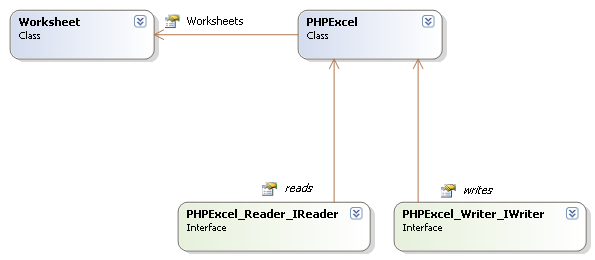
\includegraphics[scale=0.7]{skematik-phpexcel.png}  
	\caption[Arsitektur PHPExcel]{Arsitektur PHPExcel} 
	\label{fig:skematik-phpexcel} 
\end{figure}

Untuk menjalankan PHPExcel, diperlukan :
\begin{itemize}
	\item  PHP versi 5.2.0 keatas
	\item  PHP extension php\_zip diaktifkan
	\item  PHP extension php\_xml diaktifkan
	\item  PHP extension php\_gd2 diaktifkan 
\end{itemize}

\subsubsection{Membuat \textit{Spreadsheet}}
\paragraph{} Untuk membuat \textit{spreadsheet} pengguna perlu menggunakan kelas PHPExcel. Kelas PHPExcel ini merupakan bagian inti dari PHPExcel, kelas ini merepresentasikan \textit{workbook} yang akan dibuat. Pada umumnya ada dua cara untuk membuat \textit{workbook} sebagai berikut :\cite{phpexcel:14} 
\begin{enumerate}
	\item \textbf{Memuat \textit{workbook} dari file \textit{spreadsheet} yang sudah ada}.\\
Cara paling mudah untuk memuat sebuah \textit{workbook} adalah dengan memerintahkan \textit{PHPExcel IO Factory} untuk mengidentifikasi file \textit{workbook-}nya lalu memuatnya dengan cara memanggil \textit{static method} load() dari kelas "\textit{PHPExcel\_IOFactory}" . Contoh cara pemuatan \textit{workbook} di dalam kode aplikasi adalah sebagai berikut:
	\begin{lstlisting}
	$inputFileName = './sampleData/example1.xls';

	/** Load $inputFileName ke dalam obyek PHPExcel **/
	$objPHPExcel = PHPExcel_IOFactory::load($inputFileName);
	\end{lstlisting}
Method load() bekerja dengan cara mengidentifikasi terlebih dahulu tipe filenya, lalu menginstansiasi sebuah \textit{loader} untuk tipe file terkait.\textit{Loader} ini lalu digunakan untuk memuat \textit{file workbook}-nya dan menyimpan data-data lalu membentuknya ke dalam obyek PHPExcel. \cite{phpexcel:14} 
\paragraph{} Pada awalnya method load() akan memuat \textit{loader} yang dibutuhkan sesuai dari ekstensi \textit{file} \textit{workbook}, namun method ini akan memeriksa secara mendalam file tersebut sebelum memulai pemuatan \textit{workbook}-nya ke dalam obyek PHPExcel. Sebagai contoh bila sebuah file merupakan file CSV namun memiliki ekstensi .xls , maka file tersebut akan menolak \textit{loader} Excel5 yang biasanya digunakan untuk file .xls . Bila hal tersebut terjadi, maka method load() akan terus mencoba memuat workbook tersebut menggunakan \textit{loader-loader} lainnya sampai ditemukan \textit{loader} yang sesuai untuk file tersebut.  \textit{Loader} yang sudah cocok tersebut kemudian akan digunakan untuk membaca \textit{file}-nya.\cite{phpexcel:14} 
\paragraph{} Format file \textit{spreadsheet} yang didukung oleh PHPExcel adalah sebagai berikut:
\begin{itemize}
	\item BIFF (Excel5)
	\item SpreadsheetML (Excel2003XML)
	\item OfficeOpenXML (Excel2007)
	\item Open Document Format (OOCalc)
	\item Multiplan SYLK
	\item Gnumeric
	\item CSV
	\item HTML
\end{itemize}
	\item \textbf{Membuat \textit{workbook} baru secara manual}.\\
Untuk membuat \textit{workbook} baru , instansiasi obyek PHPExcel di dalam kode aplikasi.\cite{phpexcel:14} 
	\begin{lstlisting}
	$objPHPExcel = new PHPExcel();
	\end{lstlisting}
\textit{Workbook} baru yang dibuat akan memiliki satu buah \textit{worksheet}.
\end{enumerate}

\subsubsection{Mengakses Sel}
Untuk memasukan atau mengubah nilai dalam suatu sel berdasarkan koordinatnya dapat dilakukan dengan menggunakan method \textit{setCellValue()}.\cite{phpexcel:14} \\
Contoh :
\begin{lstlisting}
	// Memasukan nilai string ke sel A1
	$objPHPExcel->getActiveSheet()->setCellValue('A1','PHPExcel');

	// Memasukan nilai numerik ke sel A2
	$objPHPExcel->getActiveSheet()->setCellValue('A2',12345.6789);

	// Memasukan nilai boolean ke sel A3
	$objPHPExcel->getActiveSheet()->setCellValue('A3',TRUE);
	
	// Memasukan suato formula ke sel A4
	$objPHPExcel->getActiveSheet()->setCellValue(
	    'A4', 
	    '=IF(A3, CONCATENATE(A1," ", A2), CONCATENATE(A2," ", A1))'
	);
\end{lstlisting}
Tujuh tipe data yang didukung MS Excel :
\begin{itemize}
 	\item string
 	\item bilangan
 	\item boolean
 	\item null
 	\item formula
 	\item eror
 	\item \textit{inline string}
\end{itemize}
Ketika method \textit{setCellValue()} atu \textit{setValue()} dipanggil, PHPExcel akan memakai tipe data yang sesuai untuk tipe data null, boolean, float atau integer yang didapat dari PHP. PHPExcel juga bisa mengubah string yang dikirimkan dari PHP ke Excel menjadi tipe data yang lebih sesuai. Sebagai contoh string yang terdiri dari angka-angka saja akan diubah menjadi tipe data numerik, atau string yang memiliki awalan tanda sama dengan "=" akan dianggap sebagai formula.\cite{phpexcel:14} 

\paragraph{} Konversi-konversi tipe data tersebut ditangani oleh sebuah "\textit{value binder}" yang dapat diubah-ubah sesuai keinginan pengguna bila pengguna ingin mengatur cara-cara konversinya. PHPExcel standar juga menyediakan "\textit{advanced value binder}" yang menangani konversi-konversi yang lebih kompleks seperti mengonversi string menjadi bilangan pecahan seperi "3/4" menjadi nilai numerik (untuk kasus ini menjadi 0,75). Fitur ini berguna ketika memuat data dari csv atau memasukan nilai ke dalam sel dari \textit{database}.\cite{phpexcel:14}  \\
Beberapa format yang ditangani oleh \textit{advanced value binder} adalah sebagai berikut:
\begin{itemize}
	\item TRUE atau FALSE dikonversi menjadi boolean
	\item String yang berisi nilai numerik akan diubah menjadi bilangan
	\item Pecahan akan diubah menjadi bilangan
	\item Persentase akan diubah menjadi bilangan yang dibagi 100
	\item Tanggal dan waktu akan diubah menjadi nilai \textit{timestamp} di Excel
	\item Ketika string mengandung karakter yang memerintahkan pembautan baris baru (\\n), maka sel akan diatur menjadi menggunakan style "\textit{wrap}" 
\end{itemize}

\subsubsection{Memasukan Tanggal dan atau Waktu ke Dalam Sel}
Nilai tanggal dan waktu disimpan dalam rupa \textit{timestamp} (bilangan desimal biasa) di dalam Excel. Bilangan tersebut kemudian dibungkus oleh bilangan lain yang menentukan format penulisan tanggalnya. Jadi untuk memasukan tanggal ke dalam sel, perlu dihitung \textit{timestamp} yang benar, dan menentukan bilangan pembungkusnya.\cite{phpexcel:14} 
\begin{lstlisting}
	// Mendapatkan tanggal dan waktu saat ini
	$dateTimeNow = time();
	$excelDateValue = PHPExcel_Shared_Date::PHPToExcel( $dateTimeNow );
	// Memasukan tanggal dan waktu ke dalam sel A6
	$objPHPExcel->getActiveSheet()->setCellValue(
	    'A6', 
	    $excelDateValue
	);
	// Mengatur format bilangan pembungkus sehingga timestamp dalam Excel bisa ditampilkan dalam format yang dapat dibaca oleh manusia
	$objPHPExcel->getActiveSheet()->getStyle('A6')
	    ->getNumberFormat()
	    ->setFormatCode(
 	       PHPExcel_Style_NumberFormat::FORMAT_DATE_DATETIME
 	   );
\end{lstlisting}

\subsubsection{Memasukan Data Numerik yang Diawali Angka Nol}
\paragraph{} Pada umumnya PHPExcel secara otomatis akan mendeteksi tipe dari nilai yang dimasukan dan mengubahnya menjadi tipe data numerik di Excel. Tipe konversi ini ditangani oleh \textit{value binder}. Karena bilangan tidak memiliki awal angka nol, maka jika ada nilai numerik yang memiliki awalan angka nol (misalnya nomor telpon), maka nilai tersebut akan kehilangan angka-angka nol yang berada di depan.\cite{phpexcel:14}  \\
Untuk mencegah konversi demikian, ada beberapa cara untuk melakukannya diantaranya sebagai berikut:
\begin{enumerate}
	\item Menentukan secara manual di dalam kode agar tipe datanya tidak dikonversi ke dalam bilangan.
	\begin{lstlisting}
	// Memasukan nilai numerik ke dalam sel A8, tetapi memerintahkan PHPExcel untuk menyimpan nilai tersebut dalam tipe data String
	$objPHPExcel->getActiveSheet()->setCellValueExplicit(
	    'A8', 
	    "01513789642",
	    PHPExcel_Cell_DataType::TYPE_STRING
	);
	\end{lstlisting}
	\item Cara lainnya adalah dengan menentukan format bilangan di dalam worksheet agar menampilkan bilangan dengan awalan nol.
	\begin{lstlisting}
	// Memasukan nilai numerik ke dalam sel A9
	$objPHPExcel->getActiveSheet()->setCellValue('A9', 1513789642);
	// Menentukan format sel untuk menampilkan nilai dalam selnya berupa bilangan 11 digit dengan awalan nol
	$objPHPExcel->getActiveSheet()->getStyle('A9')
 	   ->getNumberFormat()
 	   ->setFormatCode(
  	      '00000000000'
  	  );
	\end{lstlisting}
	\item Cara kedua juga dapat digunakan untuk memisahkan digit-digit ke dalam grup agar lebih mudah dibaca.
	\begin{lstlisting}
	// Memasukan nilai numerik ke dalam sel A10
	$objPHPExcel->getActiveSheet()->setCellValue('A10', 1513789642);
	//Mengatur format sel untuk menampilkan nilai dalam selnya berupa bilangan 11 digit dengan awalan nol
	$objPHPExcel->getActiveSheet()->getStyle('A10')
    	->getNumberFormat()
    	->setFormatCode(
        	'0000-000-0000'
    );
	\end{lstlisting}
\end{enumerate}
